\documentclass[12pt]{article}
\def\activityid{F05-M-v3}\usepackage[letterpaper,margin=.65in,top=.60in,bottom=.65in]{geometry}
\usepackage[T1]{fontenc}\usepackage[default]{sourcesanspro}
\usepackage{microtype,tikz,array,tabularx,fancyhdr,amsmath}\usepackage[hidelinks]{hyperref}
\usetikzlibrary{arrows.meta,calc}
\setlength{\parindent}{0pt}\setlength{\parskip}{7pt}\setlength{\headheight}{0pt}\setlength{\footskip}{26pt}\setlength{\emergencystretch}{2em}
\pagestyle{fancy}\fancyhf{}\renewcommand{\headrulewidth}{0pt}\renewcommand{\footrulewidth}{.4pt}
\fancyfoot[L]{\scriptsize Bellingham Math Circle / Week 5 / \activityid}\fancyfoot[R]{\scriptsize \thepage}
\definecolor{ink}{gray}{.12}\definecolor{soft}{gray}{.95}\color{ink}
\newcommand{\PageTitle}[2]{{\fontsize{10}{12}\selectfont\bfseries WEEK 5\quad TOWER LAB\hfill #1\par}\vspace{3pt}{\fontsize{26}{29}\selectfont\bfseries #2\par}\vspace{2pt}}
\newcommand{\Subhead}[1]{\par\vspace{3pt}{\large\bfseries #1}\par}
\newcommand{\RuleBox}[1]{\par\begingroup\setlength{\fboxsep}{8pt}\colorbox{soft}{\parbox{\dimexpr\linewidth-16pt\relax}{#1}}\endgroup\par}
\newcommand{\WriteBox}[2]{\par\textbf{#1}\par\vspace{2pt}\begin{tikzpicture}\draw[black!40,line width=.5pt] (0,0) rectangle (\dimexpr\linewidth-.5pt\relax,#2);\end{tikzpicture}\par}
\newcommand{\Code}[1]{\texttt{#1}}

\newcommand{\StudentHeader}[1]{{\fontsize{10}{12}\selectfont\bfseries Week 5 / Tower lab / #1\par}\vspace{10pt}}
\newcommand{\Problem}[2]{\par\vspace{4pt}\textbf{Problem #1:} #2\par}
\newcommand{\RecordBox}[2]{\par #1\par\vspace{2pt}\begin{tikzpicture}\draw[black!40,line width=.5pt](0,0)rectangle(\dimexpr\linewidth-.5pt\relax,#2);\end{tikzpicture}\par}

\hypersetup{pdftitle={Week 5: Grades 2--3}}
\begin{document}
\StudentHeader{Grades 2--3}
\Problem{1}{Build each row with towers of heights 1, 2, and 3. Count the towers you can see from each end; a taller tower hides a shorter one behind it. Keep the row still when you change ends.}
\begin{center}\renewcommand{\arraystretch}{1.9}\begin{tabular}{p{2.4in}|c|c}Order, left to right & Seen from left & Seen from right\\\hline
1 2 3 &  & \\
2 1 3 &  & \\
2 3 1 &  & \\
3 2 1 &  & \\\end{tabular}\end{center}
\Problem{2}{Build a city with heights 1, 2, and 3 once in every row and once in every column. Record the heights in the left grid. Swap two whole rows of towers. Check every row and column again, then record the new city in the right grid.}
\begin{center}\begin{minipage}{.48\linewidth}\centering 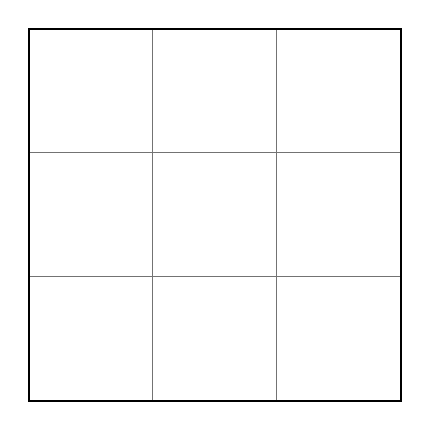
\begin{tikzpicture}[x=0.62in,y=0.62in]\draw[step=1,black!55](0,0)grid(3,3);\draw[thick](0,0)rectangle(3,3);\end{tikzpicture}\end{minipage}\hfill\begin{minipage}{.48\linewidth}\centering 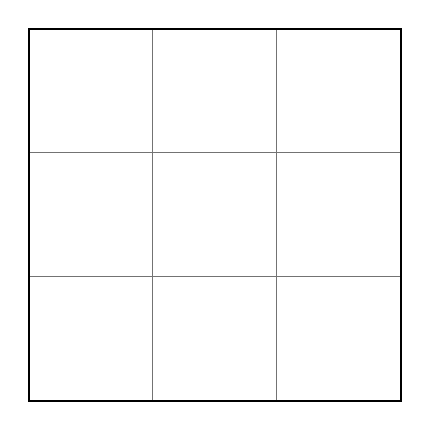
\begin{tikzpicture}[x=0.62in,y=0.62in]\draw[step=1,black!55](0,0)grid(3,3);\draw[thick](0,0)rectangle(3,3);\end{tikzpicture}\end{minipage}\end{center}
\RecordBox{The rows I swapped:}{0.45in}

\newpage
\StudentHeader{Grades 2--3}
\Problem{3}{The 3 above the first column means three towers must be visible from that end. Build a city with this clue. Record it on the left. Change the city while keeping the clue and the row and column rules true. Record a different city on the right.}
\begin{center}\begin{minipage}{.48\linewidth}\centering 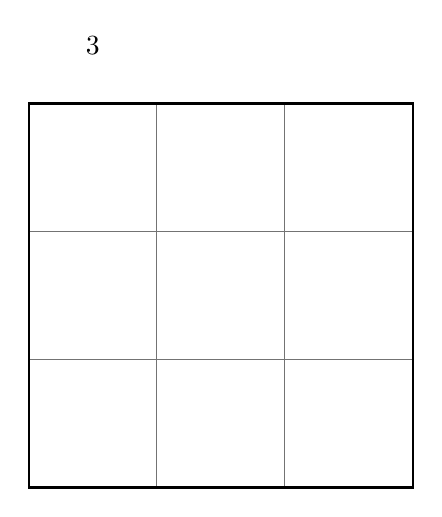
\begin{tikzpicture}[x=0.64in,y=0.64in]\draw[step=1,black!55](0,0)grid(3,3);\draw[thick](0,0)rectangle(3,3);\node at(0.5,3.45){3};\end{tikzpicture}\end{minipage}\hfill\begin{minipage}{.48\linewidth}\centering 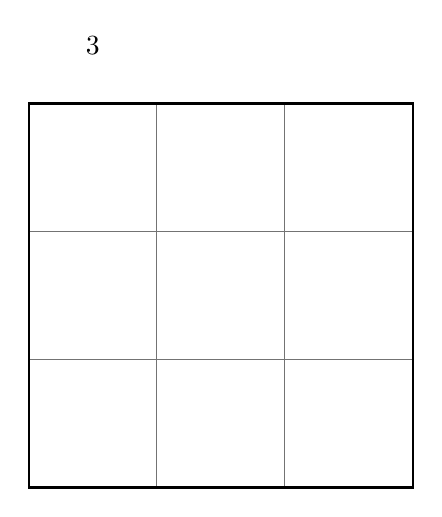
\begin{tikzpicture}[x=0.64in,y=0.64in]\draw[step=1,black!55](0,0)grid(3,3);\draw[thick](0,0)rectangle(3,3);\node at(0.5,3.45){3};\end{tikzpicture}\end{minipage}\end{center}
\Problem{4}{Copy the first column your clue requires. List the possible orders for the top row. For each top row, try to fill the rest of its city using the grids above.}
\RecordBox{First column, top to bottom:}{0.5in}
\RecordBox{Possible top rows, left to right:}{0.9in}

\newpage
\StudentHeader{Grades 2--3}
\Problem{5}{Keep the top clue 3. Add a right-hand clue of 2 on the middle row. Test both cities from Problem 3. Cross out any that break the new clue, then record a city that keeps both clues.}
\begin{center}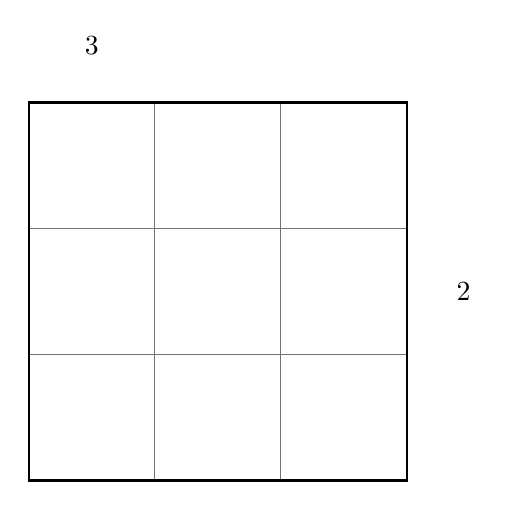
\begin{tikzpicture}[x=0.63in,y=0.63in]\draw[step=1,black!55](0,0)grid(3,3);\draw[thick](0,0)rectangle(3,3);\node at(0.5,3.45){3};\node at(3.45,1.5){2};\end{tikzpicture}\end{center}
\Problem{6}{Cover only the top clue. Build two different cities that still show two towers from the right of the middle row. Record both and check every row and column.}
\begin{center}\begin{minipage}{.48\linewidth}\centering 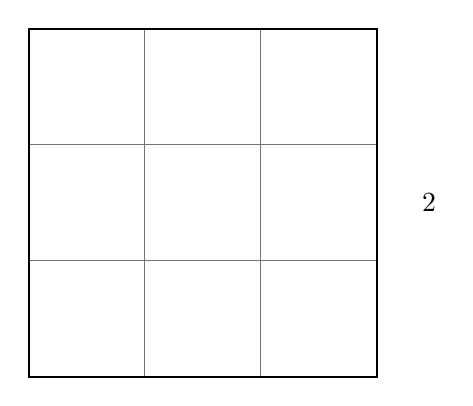
\begin{tikzpicture}[x=0.58in,y=0.58in]\draw[step=1,black!55](0,0)grid(3,3);\draw[thick](0,0)rectangle(3,3);\node at(3.45,1.5){2};\end{tikzpicture}\end{minipage}\hfill\begin{minipage}{.48\linewidth}\centering 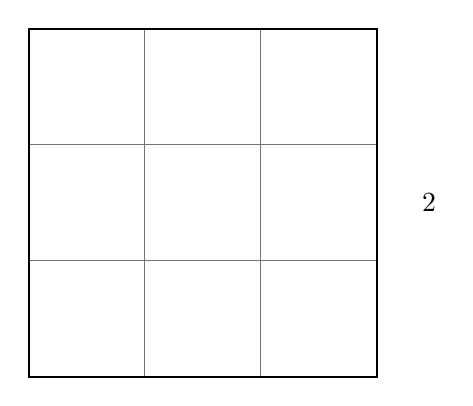
\begin{tikzpicture}[x=0.58in,y=0.58in]\draw[step=1,black!55](0,0)grid(3,3);\draw[thick](0,0)rectangle(3,3);\node at(3.45,1.5){2};\end{tikzpicture}\end{minipage}\end{center}

\end{document}
